% Options for packages loaded elsewhere
\PassOptionsToPackage{unicode}{hyperref}
\PassOptionsToPackage{hyphens}{url}
%
\documentclass[
]{article}
\usepackage{amsmath,amssymb}
\usepackage{lmodern}
\usepackage{iftex}
\ifPDFTeX
  \usepackage[T1]{fontenc}
  \usepackage[utf8]{inputenc}
  \usepackage{textcomp} % provide euro and other symbols
\else % if luatex or xetex
  \usepackage{unicode-math}
  \defaultfontfeatures{Scale=MatchLowercase}
  \defaultfontfeatures[\rmfamily]{Ligatures=TeX,Scale=1}
\fi
% Use upquote if available, for straight quotes in verbatim environments
\IfFileExists{upquote.sty}{\usepackage{upquote}}{}
\IfFileExists{microtype.sty}{% use microtype if available
  \usepackage[]{microtype}
  \UseMicrotypeSet[protrusion]{basicmath} % disable protrusion for tt fonts
}{}
\makeatletter
\@ifundefined{KOMAClassName}{% if non-KOMA class
  \IfFileExists{parskip.sty}{%
    \usepackage{parskip}
  }{% else
    \setlength{\parindent}{0pt}
    \setlength{\parskip}{6pt plus 2pt minus 1pt}}
}{% if KOMA class
  \KOMAoptions{parskip=half}}
\makeatother
\usepackage{xcolor}
\usepackage[margin=1in]{geometry}
\usepackage{color}
\usepackage{fancyvrb}
\newcommand{\VerbBar}{|}
\newcommand{\VERB}{\Verb[commandchars=\\\{\}]}
\DefineVerbatimEnvironment{Highlighting}{Verbatim}{commandchars=\\\{\}}
% Add ',fontsize=\small' for more characters per line
\usepackage{framed}
\definecolor{shadecolor}{RGB}{248,248,248}
\newenvironment{Shaded}{\begin{snugshade}}{\end{snugshade}}
\newcommand{\AlertTok}[1]{\textcolor[rgb]{0.94,0.16,0.16}{#1}}
\newcommand{\AnnotationTok}[1]{\textcolor[rgb]{0.56,0.35,0.01}{\textbf{\textit{#1}}}}
\newcommand{\AttributeTok}[1]{\textcolor[rgb]{0.77,0.63,0.00}{#1}}
\newcommand{\BaseNTok}[1]{\textcolor[rgb]{0.00,0.00,0.81}{#1}}
\newcommand{\BuiltInTok}[1]{#1}
\newcommand{\CharTok}[1]{\textcolor[rgb]{0.31,0.60,0.02}{#1}}
\newcommand{\CommentTok}[1]{\textcolor[rgb]{0.56,0.35,0.01}{\textit{#1}}}
\newcommand{\CommentVarTok}[1]{\textcolor[rgb]{0.56,0.35,0.01}{\textbf{\textit{#1}}}}
\newcommand{\ConstantTok}[1]{\textcolor[rgb]{0.00,0.00,0.00}{#1}}
\newcommand{\ControlFlowTok}[1]{\textcolor[rgb]{0.13,0.29,0.53}{\textbf{#1}}}
\newcommand{\DataTypeTok}[1]{\textcolor[rgb]{0.13,0.29,0.53}{#1}}
\newcommand{\DecValTok}[1]{\textcolor[rgb]{0.00,0.00,0.81}{#1}}
\newcommand{\DocumentationTok}[1]{\textcolor[rgb]{0.56,0.35,0.01}{\textbf{\textit{#1}}}}
\newcommand{\ErrorTok}[1]{\textcolor[rgb]{0.64,0.00,0.00}{\textbf{#1}}}
\newcommand{\ExtensionTok}[1]{#1}
\newcommand{\FloatTok}[1]{\textcolor[rgb]{0.00,0.00,0.81}{#1}}
\newcommand{\FunctionTok}[1]{\textcolor[rgb]{0.00,0.00,0.00}{#1}}
\newcommand{\ImportTok}[1]{#1}
\newcommand{\InformationTok}[1]{\textcolor[rgb]{0.56,0.35,0.01}{\textbf{\textit{#1}}}}
\newcommand{\KeywordTok}[1]{\textcolor[rgb]{0.13,0.29,0.53}{\textbf{#1}}}
\newcommand{\NormalTok}[1]{#1}
\newcommand{\OperatorTok}[1]{\textcolor[rgb]{0.81,0.36,0.00}{\textbf{#1}}}
\newcommand{\OtherTok}[1]{\textcolor[rgb]{0.56,0.35,0.01}{#1}}
\newcommand{\PreprocessorTok}[1]{\textcolor[rgb]{0.56,0.35,0.01}{\textit{#1}}}
\newcommand{\RegionMarkerTok}[1]{#1}
\newcommand{\SpecialCharTok}[1]{\textcolor[rgb]{0.00,0.00,0.00}{#1}}
\newcommand{\SpecialStringTok}[1]{\textcolor[rgb]{0.31,0.60,0.02}{#1}}
\newcommand{\StringTok}[1]{\textcolor[rgb]{0.31,0.60,0.02}{#1}}
\newcommand{\VariableTok}[1]{\textcolor[rgb]{0.00,0.00,0.00}{#1}}
\newcommand{\VerbatimStringTok}[1]{\textcolor[rgb]{0.31,0.60,0.02}{#1}}
\newcommand{\WarningTok}[1]{\textcolor[rgb]{0.56,0.35,0.01}{\textbf{\textit{#1}}}}
\usepackage{graphicx}
\makeatletter
\def\maxwidth{\ifdim\Gin@nat@width>\linewidth\linewidth\else\Gin@nat@width\fi}
\def\maxheight{\ifdim\Gin@nat@height>\textheight\textheight\else\Gin@nat@height\fi}
\makeatother
% Scale images if necessary, so that they will not overflow the page
% margins by default, and it is still possible to overwrite the defaults
% using explicit options in \includegraphics[width, height, ...]{}
\setkeys{Gin}{width=\maxwidth,height=\maxheight,keepaspectratio}
% Set default figure placement to htbp
\makeatletter
\def\fps@figure{htbp}
\makeatother
\setlength{\emergencystretch}{3em} % prevent overfull lines
\providecommand{\tightlist}{%
  \setlength{\itemsep}{0pt}\setlength{\parskip}{0pt}}
\setcounter{secnumdepth}{-\maxdimen} % remove section numbering
\ifLuaTeX
  \usepackage{selnolig}  % disable illegal ligatures
\fi
\IfFileExists{bookmark.sty}{\usepackage{bookmark}}{\usepackage{hyperref}}
\IfFileExists{xurl.sty}{\usepackage{xurl}}{} % add URL line breaks if available
\urlstyle{same} % disable monospaced font for URLs
\hypersetup{
  pdftitle={Assignment2},
  pdfauthor={Sean Anselmo},
  hidelinks,
  pdfcreator={LaTeX via pandoc}}

\title{Assignment2}
\author{Sean Anselmo}
\date{2024-01-24}

\begin{document}
\maketitle

\hypertarget{question-1}{%
\subsection{Question 1}\label{question-1}}

Billy purchases one 6-49 lottery ticket every week and keeps track of
the number of ``matches'''' he has on each of his tickets. To be clear,
a ``match'' will occur when a number on his ticket matches a number that
appears in the winning combination. A random variable X that keeps track
of the number of matching numbers Billy experiences per week has the
probability distribution function with a mean and standard deviation of
**P(X=x)= choose(6,x)*choose(43,6-x)/choose(49,6)
x=0,1,2,3,4,5,6.\textbf{ }E(X) = μX = 36/49 = 0.7347\textbf{ }SD(X) = σX
= 0.75998≈ 0.76**

Billy claims that in a year (52 weeks), on average, he manages to have
at least one matching number on his 6-49 ticket. What do you think about
Billy's claim? Provide a brief commentary about Billy's claim using your
current knowledge of statistics and probability theory.

\begin{Shaded}
\begin{Highlighting}[]
\CommentTok{\#Calculate the odds he draws P(x=0) and then subtract that from 1.}
\NormalTok{PxIs0 }\OtherTok{=}\NormalTok{ (}\FunctionTok{choose}\NormalTok{(}\DecValTok{6}\NormalTok{,}\DecValTok{0}\NormalTok{)}\SpecialCharTok{*}\FunctionTok{choose}\NormalTok{(}\DecValTok{43}\NormalTok{,}\DecValTok{6}\NormalTok{))}\SpecialCharTok{/}\FunctionTok{choose}\NormalTok{(}\DecValTok{49}\NormalTok{,}\DecValTok{6}\NormalTok{)}
\NormalTok{AtLeastOne }\OtherTok{=} \DecValTok{1} \SpecialCharTok{{-}}\NormalTok{ PxIs0}\SpecialCharTok{\^{}}\DecValTok{52} \CommentTok{\#Do it 52 times for a year}
\end{Highlighting}
\end{Shaded}

\textbf{Answer to Q1} Billy's chances of getting 0 numbers on his card
for 52 weeks straight is nearing 0, meaning he was correct in assuming
that he will on average get at least one number on his card in a years
time. This is compounded by his expected value being 0.7347, and his
standard deviation being 0.76 This allows us to use the Central Limit
Theorem to assume that x is very likely to fall at or above 1 for at
minimum one week in the 52 week span. With that being said, E(X) is less
than one meaning he is unlikely to get a ticket each week.

\hypertarget{question-2}{%
\subsection{Question 2}\label{question-2}}

A common measure of toxicity for any pollutant is the concentration of
the pollutant that will kill half of the test species in a given amount
of time (usually about 96 hours for the fish species). This measurement
is called the LC50, which refers to the lethal concentration killing
50\% of the test species).

The Environmental Protection Agency has collected data on LC50
measurements for certain chemicals likely to be found in freshwater and
lakes. For a certain species of fish, the LC50 measurements (in parts
per million) for DDT in 12 experiments to determine the LC50 ``dose''
are

\textbf{16,5,21,19,10,5,8,2,7,2,4,9}

a)Use R studio to create the bootstrap distribution of the sample mean
X¯Boot,LC50. Use 2000 ``bootstraps'' in your work, and display the
distribution.

b)From your result in (a), compute the 95\% bootstrap (percentile)
confidence interval for μLC50, the mean LC50 measurement for DDT.

c)Repeat your estimation of μLC50, using the ``other'' confidence
interval covered in Data 602. In the context of these data, interpret
the meaning of the confidence interval. State any conditions/assumptions
that are required in the computation of this confidence interval.

d)Compare your results in parts (b) and (c). If you were to report one
of these confidence intervals, which would you report? Explain your
answer.

\begin{Shaded}
\begin{Highlighting}[]
\NormalTok{data }\OtherTok{\textless{}{-}} \FunctionTok{c}\NormalTok{(}\DecValTok{16}\NormalTok{,}\DecValTok{5}\NormalTok{,}\DecValTok{21}\NormalTok{,}\DecValTok{19}\NormalTok{,}\DecValTok{10}\NormalTok{,}\DecValTok{5}\NormalTok{,}\DecValTok{8}\NormalTok{,}\DecValTok{2}\NormalTok{,}\DecValTok{7}\NormalTok{,}\DecValTok{2}\NormalTok{,}\DecValTok{4}\NormalTok{,}\DecValTok{9}\NormalTok{)}

\FunctionTok{set.seed}\NormalTok{(}\DecValTok{45}\NormalTok{)}
\NormalTok{Q2bootstrap }\OtherTok{\textless{}{-}} \FunctionTok{do}\NormalTok{(}\DecValTok{2000}\NormalTok{)}\SpecialCharTok{*}\FunctionTok{mean}\NormalTok{(}\FunctionTok{resample}\NormalTok{(data,}\AttributeTok{replace =} \ConstantTok{TRUE}\NormalTok{))}

\NormalTok{Q2bootstrap\_data\_frame }\OtherTok{\textless{}{-}} \FunctionTok{data.frame}\NormalTok{(}\AttributeTok{means =} \FunctionTok{unlist}\NormalTok{(Q2bootstrap))}
\FunctionTok{ggplot}\NormalTok{(Q2bootstrap\_data\_frame, }\FunctionTok{aes}\NormalTok{(}\AttributeTok{x=}\NormalTok{means))}\SpecialCharTok{+}
  \FunctionTok{geom\_histogram}\NormalTok{(}\AttributeTok{color =} \StringTok{\textquotesingle{}steelblue\textquotesingle{}}\NormalTok{, }\AttributeTok{fill =} \StringTok{\textquotesingle{}grey\textquotesingle{}}\NormalTok{)}\SpecialCharTok{+}
  \FunctionTok{xlab}\NormalTok{(}\StringTok{"Bootstrap Sample Mean for LC50 Measurements of DDT Usage"}\NormalTok{)}\SpecialCharTok{+}
  \FunctionTok{ggtitle}\NormalTok{(}\StringTok{"Question 2a) Bootstrap Distribution"}\NormalTok{)}
\end{Highlighting}
\end{Shaded}

\begin{verbatim}
## `stat_bin()` using `bins = 30`. Pick better value with `binwidth`.
\end{verbatim}

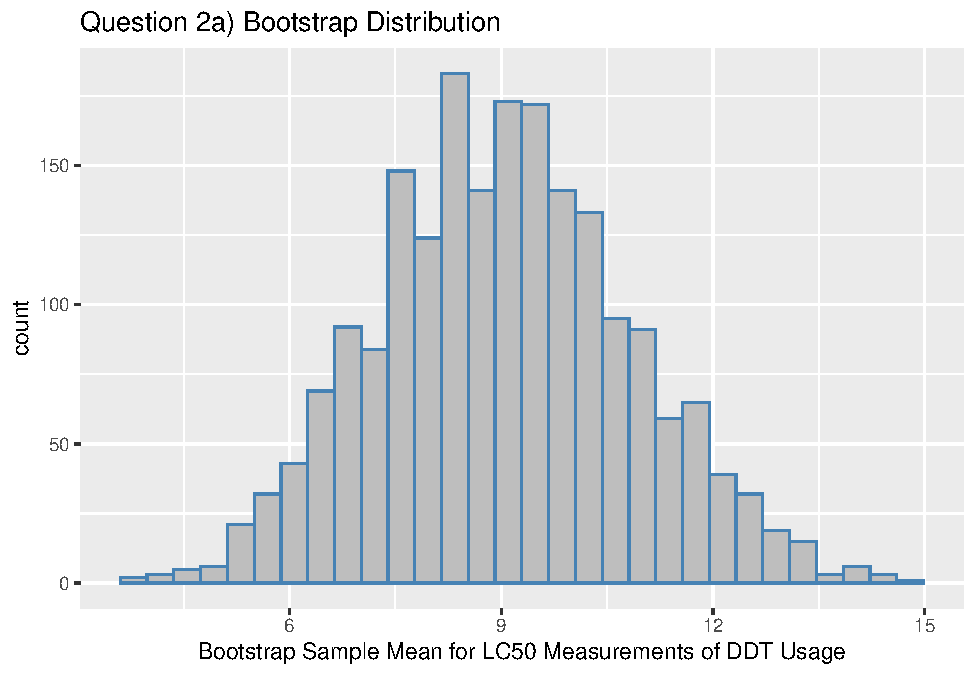
\includegraphics{Assignment2_files/figure-latex/Q2-1.pdf}

\begin{Shaded}
\begin{Highlighting}[]
\NormalTok{Q2b }\OtherTok{=} \FunctionTok{quantile}\NormalTok{(Q2bootstrap}\SpecialCharTok{$}\NormalTok{mean,}\FunctionTok{c}\NormalTok{(}\FloatTok{0.025}\NormalTok{,}\FloatTok{0.975}\NormalTok{))}

\NormalTok{ParaMean }\OtherTok{=} \FunctionTok{mean}\NormalTok{(data)}
\NormalTok{ParaSD }\OtherTok{=} \FunctionTok{sd}\NormalTok{(data)}

\NormalTok{length }\OtherTok{=} \FunctionTok{length}\NormalTok{(data)}

\NormalTok{ParaSem }\OtherTok{=}\NormalTok{ ParaSD}\SpecialCharTok{/}\FunctionTok{sqrt}\NormalTok{(length)}
\NormalTok{t }\OtherTok{=} \FunctionTok{qt}\NormalTok{(}\FloatTok{0.975}\NormalTok{,length}\DecValTok{{-}1}\NormalTok{)}

\NormalTok{moe }\OtherTok{=}\NormalTok{ t}\SpecialCharTok{*}\NormalTok{ParaSem}

\NormalTok{ParaUpper }\OtherTok{=}\NormalTok{ ParaMean }\SpecialCharTok{+}\NormalTok{ moe}
\NormalTok{ParaLower }\OtherTok{=}\NormalTok{ ParaMean }\SpecialCharTok{{-}}\NormalTok{ moe}
\end{Highlighting}
\end{Shaded}

\textbf{Answer for Question 2b} The upper and lower bounds for out 95\%
confidence interval for the LC50 Measurement of DDT is
\textbf{5.6666667, 12.5854167}. This means we are 95\% sure the mean
LC50 values lie between 5.50 and 12.75.

\textbf{Answer for Question 2c} The parametric approach yielded an upper
limit of \textbf{13.0818597} and a lower limit of \textbf{4.9181403}. We
are 95\% certain the mean of LC50 use was between 4.08 and 4.92. For the
parametric approach we assumed the data to be normally distributed, and
that the sampling was random and independant.

\textbf{Answer for Question 2d} I would use the answer from 2b, the
bootstrap approach. This is because since it is a small population, and
we do not know how the samples are distributed or the standard
deviation. The bootstrap approach makes less assumptions about the data
as a whole, which is why it is the more robust apporach to determining
the confidence interval.

\hypertarget{question-3}{%
\subsection{Question 3}\label{question-3}}

Does one's educational level influence their opinion about vaccinations?
A recent Angus Reid survey was taken. Each person sampled was asked to
respond to the statement ``The science around vaccinations isn't
clear.'' Respondents either ``strongly agree'', ``moderately agree'',
``moderately disagree'', or ``strongly disagree''. The sample was
partitioned by level of education. There were \textbf{n=670} respondents
who's highest level of education was high school or less, of which 348
``disagreed'' (moderately disagree or stongly disagree). There were also
\textbf{n=376} who's highest level of education was at least an
undergraduate university education. Of these, 274 disagreed.

a)Consider the population consisting of all persons, who's highest level
of education was high school or less and the bootstrap statistic
pˆBoot,HS . Using 1000 iterations/replications, create a bootstrap
distribution of pˆHS. Display your distribution.

b)Now consider a different population that consists of all persons who's
highest level of education was at least an undergraduate degree. Repeat
part (a), creating a bootstrap distribution for pˆBoot,Uni. (Again,
display your distribution).

c)You wish to estimate pUni−pHS, the difference between the proportion
of all university-educated Canadians who disagree that the science of
vaccinations isn't clear and the proportion of all Canadians who's
highest level of completed education is high school who believe the
same. You wish to have 95\% confidence in your result. Think about the
code you created to generate the bootstrap distributions on parts (a)
and (b). Modify the code to you created in parts (a) and (b) to create a
distribution of the bootstrap statistic pˆUni−pˆHS.

d)Consider your finding in part (c). Compute the 95\% bootstrap
percentile confidence interval for pUni−pHs. From your result, does the
proportion of persons with at most a high school education who disagree
the science around vaccinations isn't clear greater than the similar
proportion of persons with at least an undergraduate university degree?
Write a paragraph that supports your answer.

\begin{Shaded}
\begin{Highlighting}[]
\NormalTok{HighSchool }\OtherTok{=} \DecValTok{670}
\NormalTok{HighSchoolDisagree }\OtherTok{=} \DecValTok{348}

\NormalTok{data }\OtherTok{\textless{}{-}} \FunctionTok{c}\NormalTok{(}\FunctionTok{rep}\NormalTok{(}\DecValTok{1}\NormalTok{, HighSchoolDisagree), }\FunctionTok{rep}\NormalTok{(}\DecValTok{0}\NormalTok{, HighSchool}\SpecialCharTok{{-}}\NormalTok{HighSchoolDisagree))}
\NormalTok{Q3aBootstrap }\OtherTok{\textless{}{-}} \FunctionTok{do}\NormalTok{(}\DecValTok{1000}\NormalTok{)}\SpecialCharTok{*}\FunctionTok{mean}\NormalTok{(}\FunctionTok{resample}\NormalTok{(data,}\AttributeTok{replace =} \ConstantTok{TRUE}\NormalTok{))}

\FunctionTok{ggplot}\NormalTok{(Q3aBootstrap, }\FunctionTok{aes}\NormalTok{(}\AttributeTok{x=}\NormalTok{mean))}\SpecialCharTok{+}
  \FunctionTok{geom\_histogram}\NormalTok{(}\AttributeTok{color =} \StringTok{\textquotesingle{}steelblue\textquotesingle{}}\NormalTok{, }\AttributeTok{fill =} \StringTok{\textquotesingle{}orange\textquotesingle{}}\NormalTok{, }\AttributeTok{binwidth =} \FloatTok{0.01}\NormalTok{)}\SpecialCharTok{+}
  \FunctionTok{xlab}\NormalTok{(}\StringTok{"Bootstrap Sample Mean for HighSchool Educated Opinions on Vaccines"}\NormalTok{)}\SpecialCharTok{+}
  \FunctionTok{ggtitle}\NormalTok{(}\StringTok{"Question 3a) Bootstrap Distribution"}\NormalTok{)}
\end{Highlighting}
\end{Shaded}

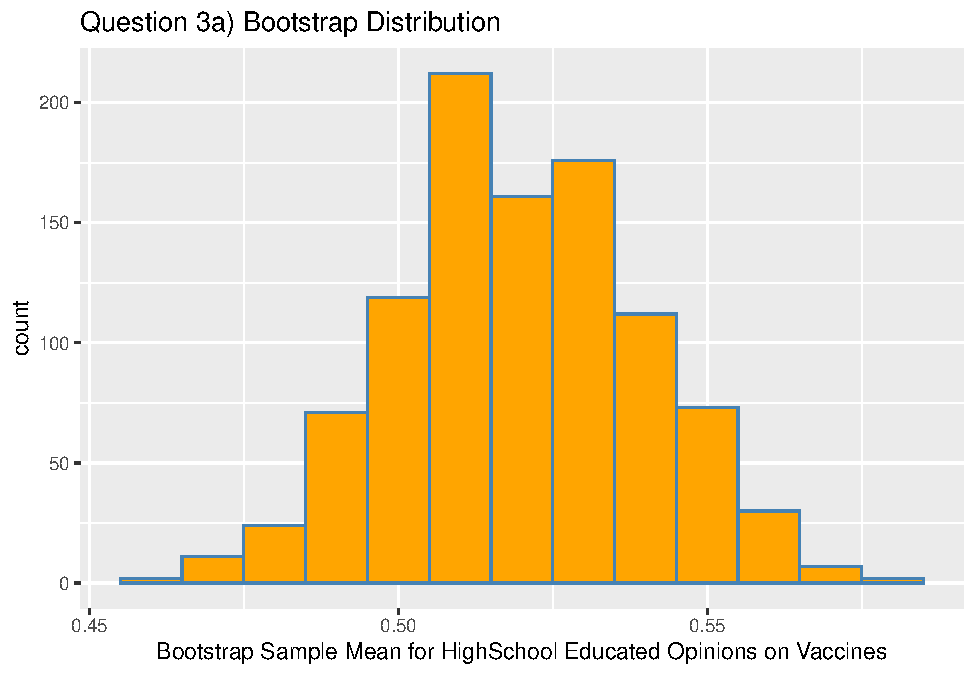
\includegraphics{Assignment2_files/figure-latex/Q3-1.pdf}

\begin{Shaded}
\begin{Highlighting}[]
\NormalTok{dataB }\OtherTok{\textless{}{-}} \FunctionTok{c}\NormalTok{(}\FunctionTok{rep}\NormalTok{(}\DecValTok{1}\NormalTok{, }\DecValTok{274}\NormalTok{),}\FunctionTok{rep}\NormalTok{(}\DecValTok{0}\NormalTok{,}\DecValTok{376{-}274}\NormalTok{))}
\NormalTok{Q3bBootstrap }\OtherTok{\textless{}{-}} \FunctionTok{do}\NormalTok{ (}\DecValTok{1000}\NormalTok{)}\SpecialCharTok{*}\FunctionTok{mean}\NormalTok{(}\FunctionTok{resample}\NormalTok{(dataB, }\AttributeTok{replace =} \ConstantTok{TRUE}\NormalTok{))}

\FunctionTok{ggplot}\NormalTok{(Q3bBootstrap, }\FunctionTok{aes}\NormalTok{(}\AttributeTok{x=}\NormalTok{mean))}\SpecialCharTok{+}
  \FunctionTok{geom\_histogram}\NormalTok{(}\AttributeTok{color =} \StringTok{\textquotesingle{}steelblue\textquotesingle{}}\NormalTok{, }\AttributeTok{fill =} \StringTok{\textquotesingle{}pink\textquotesingle{}}\NormalTok{, }\AttributeTok{binwidth =} \FloatTok{0.01}\NormalTok{)}\SpecialCharTok{+}
  \FunctionTok{xlab}\NormalTok{(}\StringTok{"Bootstrap Sample Mean for College Educated Opinions on Vaccines"}\NormalTok{)}\SpecialCharTok{+}
  \FunctionTok{ggtitle}\NormalTok{(}\StringTok{"Question 3b) Bootstrap Distribution"}\NormalTok{)}
\end{Highlighting}
\end{Shaded}

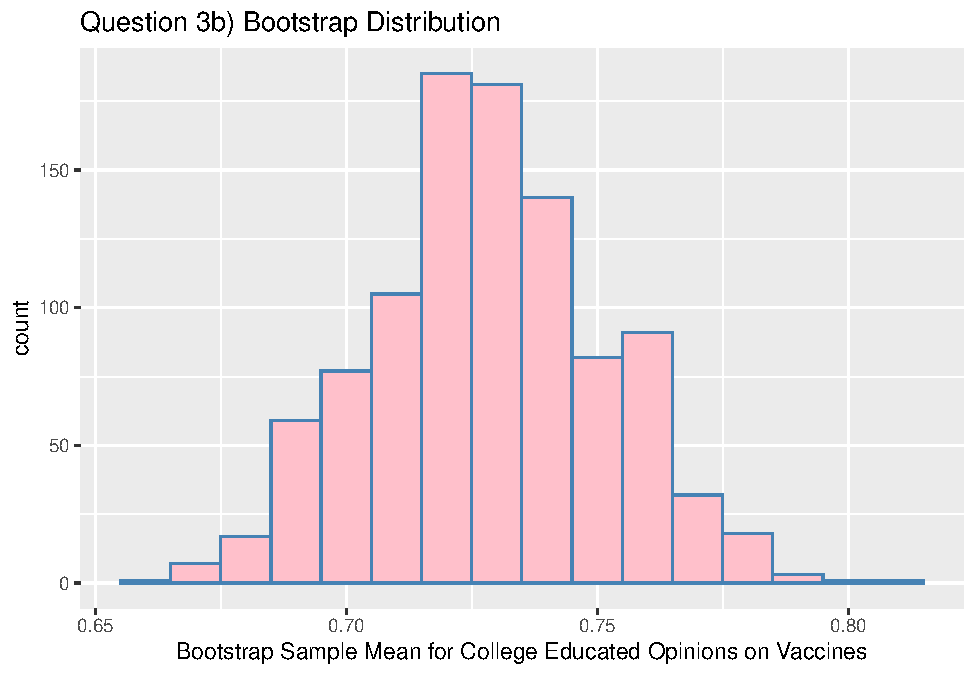
\includegraphics{Assignment2_files/figure-latex/Q3-2.pdf}

\begin{Shaded}
\begin{Highlighting}[]
\NormalTok{meansHS }\OtherTok{\textless{}{-}} \FunctionTok{unlist}\NormalTok{(Q3aBootstrap}\SpecialCharTok{$}\NormalTok{mean)}
\NormalTok{meansCollege }\OtherTok{\textless{}{-}} \FunctionTok{unlist}\NormalTok{(Q3bBootstrap}\SpecialCharTok{$}\NormalTok{mean)}

\NormalTok{Q3cBootstrap }\OtherTok{\textless{}{-}}\NormalTok{ meansCollege }\SpecialCharTok{{-}}\NormalTok{ meansHS}

\NormalTok{Q3cBootstrap\_data\_frame }\OtherTok{\textless{}{-}} \FunctionTok{data.frame}\NormalTok{(}\AttributeTok{mean =}\NormalTok{ Q3cBootstrap)}


\FunctionTok{ggplot}\NormalTok{(Q3cBootstrap\_data\_frame, }\FunctionTok{aes}\NormalTok{(}\AttributeTok{x=}\NormalTok{mean))}\SpecialCharTok{+}
  \FunctionTok{geom\_histogram}\NormalTok{(}\AttributeTok{color =} \StringTok{\textquotesingle{}steelblue\textquotesingle{}}\NormalTok{, }\AttributeTok{fill =} \StringTok{\textquotesingle{}coral\textquotesingle{}}\NormalTok{, }\AttributeTok{binwidth =} \FloatTok{0.01}\NormalTok{)}\SpecialCharTok{+}
  \FunctionTok{xlab}\NormalTok{(}\StringTok{"PhatUni {-} PhatHS"}\NormalTok{)}\SpecialCharTok{+}
  \FunctionTok{ggtitle}\NormalTok{(}\StringTok{"Question 3c) Bootstrap Distribution"}\NormalTok{)}
\end{Highlighting}
\end{Shaded}

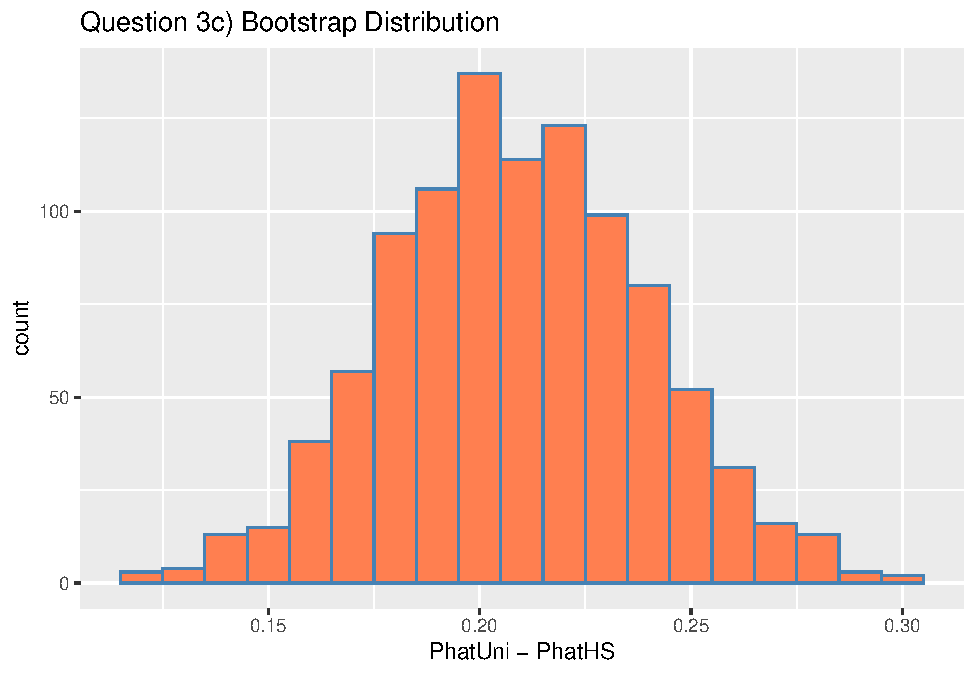
\includegraphics{Assignment2_files/figure-latex/Q3-3.pdf}

\begin{Shaded}
\begin{Highlighting}[]
\NormalTok{Q3d }\OtherTok{=} \FunctionTok{quantile}\NormalTok{(Q3cBootstrap,}\FunctionTok{c}\NormalTok{(}\FloatTok{0.025}\NormalTok{,}\FloatTok{0.975}\NormalTok{))}
\end{Highlighting}
\end{Shaded}

\textbf{Answer for Question 3d:} The 95\% confidence interal for pUni -
pHS is 0.15, 0.267. Since the interaval is above 0, we can determine
that there is a significant difference between the two groups. This
difference is represented by the proportion of individuals with at most
a highschool education who disagree with the clairty of vaccine science
(pHS) is between 15\% and 26.7\% greater than the proportion of
individuals with at least a university degree who disagree. This means
we are 95\% sure there is an actual significant difference between these
two popultions, and the difference observed is not due to random chance.

\hypertarget{question-4}{%
\subsection{Question 4}\label{question-4}}

Nanos research recently completed a survey of \textbf{n=1000} Canadians
aged 18 years of age or older, asking each ``what is your most important
national issue of concern?'' 163 responded ``Inflation'', 149 responded
``Environment'', 131 responded ``Jobs/Economy''. Those were the Top
Three.

a)Compute a 95\% confidence interval for \textbf{pInflation} , the
proportion of all Canadians aged 18 years or older for whom
``Inflation'' is the most important national concern.

b)Similar to your work in Question 4(a), create the distribution of the
bootstrap statistic \textbf{pˆBoot,Inflation} and a 95\% bootstrap
percentile confidence interval for \textbf{pInflation}.

c)A similar survey of Canadians in August 2023 - a little over a month
ago - suggested that the proportion of all Canadians who identified
``Inflation'' as the most important national concern was
\textbf{pInflation,Aug\_23=0.13}

d)From your results in (a) and (b), can you infer that the proportion of
all Canadians who believe ``Inflation'' is the most important national
issue has increased since August of this year? Why or why not? Ensure
you invoke a statistical justification.

\begin{Shaded}
\begin{Highlighting}[]
\NormalTok{n }\OtherTok{=} \DecValTok{1000}
\NormalTok{nInflation }\OtherTok{=} \DecValTok{163}
\NormalTok{nEnviroment }\OtherTok{=} \DecValTok{149}
\NormalTok{nEconomy }\OtherTok{=} \DecValTok{131}

\NormalTok{pHatInflation }\OtherTok{=}\NormalTok{ nInflation}\SpecialCharTok{/}\NormalTok{n}
\NormalTok{seInflation }\OtherTok{=} \FunctionTok{sqrt}\NormalTok{(pHatInflation}\SpecialCharTok{*}\NormalTok{(}\DecValTok{1}\SpecialCharTok{{-}}\NormalTok{pHatInflation)}\SpecialCharTok{/}\NormalTok{n)}

\NormalTok{z }\OtherTok{=} \FunctionTok{qnorm}\NormalTok{(}\FloatTok{0.975}\NormalTok{)}

\NormalTok{moe }\OtherTok{=}\NormalTok{ z}\SpecialCharTok{*}\NormalTok{seInflation}

\NormalTok{lower }\OtherTok{=}\NormalTok{ (pHatInflation}\SpecialCharTok{{-}}\NormalTok{moe)}\SpecialCharTok{*}\DecValTok{100}
\NormalTok{upper }\OtherTok{=}\NormalTok{ (pHatInflation}\SpecialCharTok{+}\NormalTok{moe)}\SpecialCharTok{*}\DecValTok{100}

\FunctionTok{set.seed}\NormalTok{(}\DecValTok{45}\NormalTok{)}
\NormalTok{dataQ4 }\OtherTok{=} \FunctionTok{c}\NormalTok{(}\FunctionTok{rep}\NormalTok{(}\DecValTok{1}\NormalTok{, nInflation), }\FunctionTok{rep}\NormalTok{(}\DecValTok{0}\NormalTok{, n}\SpecialCharTok{{-}}\NormalTok{nInflation))}
\NormalTok{Q4bootstrap }\OtherTok{=} \FunctionTok{do}\NormalTok{(}\DecValTok{1000}\NormalTok{)}\SpecialCharTok{*}\FunctionTok{mean}\NormalTok{(}\FunctionTok{resample}\NormalTok{(dataQ4, }\AttributeTok{replace =} \ConstantTok{TRUE}\NormalTok{))}

\NormalTok{Q4B }\OtherTok{=} \FunctionTok{quantile}\NormalTok{(Q4bootstrap}\SpecialCharTok{$}\NormalTok{mean, }\AttributeTok{probs =} \FunctionTok{c}\NormalTok{(}\FloatTok{0.025}\NormalTok{,}\FloatTok{0.975}\NormalTok{))}
\end{Highlighting}
\end{Shaded}

\textbf{Answer for Question 4a)} The lower bound for the 95\% confidence
interval for Inflation concerns is \textbf{14.0106899\%}, and the upper
bound is \textbf{18.5893101\%}

\textbf{Answer for Question 4b)} 0.141, 0.187

\textbf{Answer for Question 4c)} We are 95\% sure the number of
Canadians who identify Inflation as their primary concern has risen
since August. This is because the pInfaltion(Aug 2023) was
\textbf{13\%}, which is lower than our lower bound of \textbf{14\%}.
\textbf{13\%} also does not fall within our bootstrap method lower bound
of \textbf{14.1}, further coorberating our reasoning. Since it does lie
within our confidence interval, we can make this claim with 95\%
certainty.

\hypertarget{question-5}{%
\subsection{Question 5}\label{question-5}}

A national survey 4 of \textbf{n=399} ``Gen Z''-ers - someone who is
born in the years 1996 - 2010 (inclusive) was taken. Each was then asked
the following question: ``If a federal election were held tomorrow,
which one of the following parties would you vote for in your
constituency?'' The results?

128 responded ``Conservative'' (Conservative Party of Canada) 96
responded ``Liberal'' (Liberal Party of Canada) 104 responded ``NDP''
(New Democratic Party of Canada)

Respondents were provided with a few more ``closed options'', including
the Bloc Quebecois, People's Party, and Green Party.

a)Compute the 95\% confidence interval for \textbf{pCon}, the proportion
of all Gen Z-ers in Canada that will vote for their respective
Conservative Member of Parliament candidate/constituency, in an election
were ``held tomorrow''.

b)Consider the bootstrap statistic \textbf{p˜Con=XCon+2/(399+4)}. Write
the R code that will generate a bootstrap distribution for
\textbf{p˜Con}. Use 1000 as the number of replications/iterations.

c)From your result in part (b), compute a 95\% bootstrap confidence
interval for \textbf{pCon}.

d)Consider your results in parts (a) and (c). Compare the two results.
If you had to pick one as the ``best'' estimate for the unknown value of
\textbf{pCon}, which one would you select? Provide a justification for
your choice.

\begin{Shaded}
\begin{Highlighting}[]
\NormalTok{n }\OtherTok{=} \DecValTok{399}
\NormalTok{nLiberal }\OtherTok{=} \DecValTok{96}
\NormalTok{nConservative }\OtherTok{=} \DecValTok{128}
\NormalTok{nNDP }\OtherTok{=} \DecValTok{104}

\NormalTok{pHatCon }\OtherTok{=}\NormalTok{ nConservative}\SpecialCharTok{/}\NormalTok{n}
\NormalTok{seCon }\OtherTok{=} \FunctionTok{sqrt}\NormalTok{(pHatCon}\SpecialCharTok{*}\NormalTok{(}\DecValTok{1}\SpecialCharTok{{-}}\NormalTok{pHatCon)}\SpecialCharTok{/}\NormalTok{n)}

\NormalTok{z }\OtherTok{=} \FunctionTok{qnorm}\NormalTok{(}\FloatTok{0.975}\NormalTok{)}

\NormalTok{moe }\OtherTok{=}\NormalTok{ z}\SpecialCharTok{*}\NormalTok{seCon}

\NormalTok{lowerCon }\OtherTok{=}\NormalTok{ (pHatCon}\SpecialCharTok{{-}}\NormalTok{moe)}\SpecialCharTok{*}\DecValTok{100}
\NormalTok{upperCon }\OtherTok{=}\NormalTok{ (pHatCon}\SpecialCharTok{+}\NormalTok{moe)}\SpecialCharTok{*}\DecValTok{100}

\CommentTok{\#Code Answer for Q5B}
\FunctionTok{set.seed}\NormalTok{(}\DecValTok{45}\NormalTok{)}
\NormalTok{dataQ5 }\OtherTok{\textless{}{-}} \FunctionTok{c}\NormalTok{(}\FunctionTok{rep}\NormalTok{(}\DecValTok{1}\NormalTok{, nConservative), }\FunctionTok{rep}\NormalTok{(}\DecValTok{0}\NormalTok{, n }\SpecialCharTok{{-}}\NormalTok{ nConservative))}
\NormalTok{Q5bootstrap }\OtherTok{\textless{}{-}} \FunctionTok{replicate}\NormalTok{(}\DecValTok{1000}\NormalTok{, \{}
\NormalTok{  sample\_mean }\OtherTok{\textless{}{-}} \FunctionTok{mean}\NormalTok{(}\FunctionTok{resample}\NormalTok{(dataQ5, }\AttributeTok{replace =} \ConstantTok{TRUE}\NormalTok{))}

\NormalTok{  (sample\_mean }\SpecialCharTok{*}\NormalTok{ n }\SpecialCharTok{+} \DecValTok{2}\NormalTok{) }\SpecialCharTok{/}\NormalTok{ (n }\SpecialCharTok{+} \DecValTok{4}\NormalTok{)}
\NormalTok{\})}

\NormalTok{Q5bootstrap\_data\_frame }\OtherTok{=} \FunctionTok{data.frame}\NormalTok{(}\AttributeTok{means =} \FunctionTok{unlist}\NormalTok{(Q5bootstrap))}

\NormalTok{Q5C }\OtherTok{=} \FunctionTok{quantile}\NormalTok{(Q5bootstrap\_data\_frame}\SpecialCharTok{$}\NormalTok{means, }\AttributeTok{probs =} \FunctionTok{c}\NormalTok{(}\FloatTok{0.025}\NormalTok{, }\FloatTok{0.975}\NormalTok{))}


\FunctionTok{ggplot}\NormalTok{(Q5bootstrap\_data\_frame, }\FunctionTok{aes}\NormalTok{(}\AttributeTok{x=}\NormalTok{means))}\SpecialCharTok{+}
  \FunctionTok{geom\_histogram}\NormalTok{(}\AttributeTok{color =} \StringTok{\textquotesingle{}steelblue\textquotesingle{}}\NormalTok{, }\AttributeTok{fill =} \StringTok{\textquotesingle{}grey\textquotesingle{}}\NormalTok{, }\AttributeTok{binwidth =} \FloatTok{0.01}\NormalTok{)}\SpecialCharTok{+}
  \FunctionTok{xlab}\NormalTok{(}\StringTok{"Bootstrap Distribution for Gen Z who would Vote Conservative"}\NormalTok{)}\SpecialCharTok{+}
  \FunctionTok{ggtitle}\NormalTok{(}\StringTok{"Question 5a) Bootstrap Distribution"}\NormalTok{)}
\end{Highlighting}
\end{Shaded}

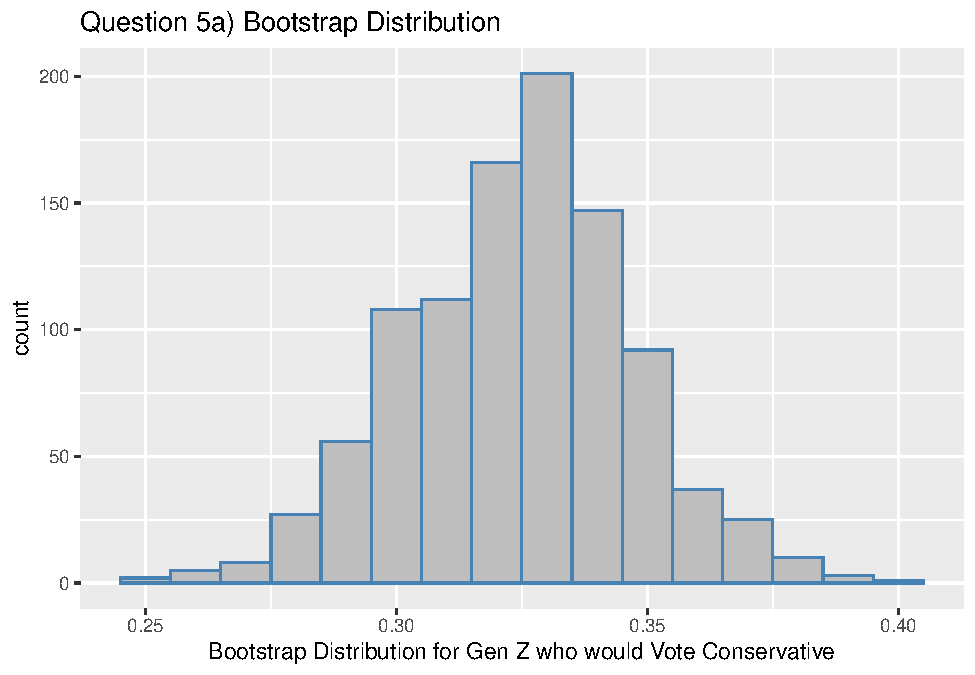
\includegraphics{Assignment2_files/figure-latex/Q5-1.pdf} \textbf{Answer
for Question 5a)} The lower bound for the 95\% confidence interval for
Gen Z'ers who would vote conservative is \textbf{27.5000645\%}, and the
upper bound is \textbf{36.6603365\%}

\textbf{Answer for Question 5c)} 0.2779156, 0.369727

\textbf{Answer for Question 5d)} We should use the bootstrap approach
from part 5c. There is a sufficient population number, and we are not
sure of the distribution to use the parametric approach. Unlike in
Question 2, we have a sufficient n value and therefore we should use the
bootstrap approach, but the decision is close.

\end{document}
